\scanpage{60}
\mspage{\deleted{\unsure{3|5}} 4}

Le fait que ça donne bien une structure conforme à bord \deleted{équivaut} (qui automatiquement, \unsure{redonnera|redonne} \deleted{naissance} \inserted{avec $K$} à la structure conforme à bord $\widetilde X$ de départ) équivaut aux \deleted{lemme suivant :} \inserted{deux cas particuliers suivants}

\deleted{\uline{Lemme 3}

a) Soit $\sigma$ un homéomorphisme rectifiable (ou plus régulier que ça ?) de $[0,1]$ sur lui \deleted{\unsure{ou|même}}, avec $\sigma(0)=0$, $\sigma(1)=1$, alors il existe une \deleted{courbe} \inserted{partie fermée} $K\subset H\cap\mathbb D^\circ$, \deleted{bornée contenant 0, telle que $K\smallsetminus\{0\}$ soit contenue dans $\operatorname{Int} H$} \inserted{avec $K\cap\partial H=\{0\}$}, $K$ étant un intervalle demi-ouvert d'extrémité 0, qui partage $H\cap\mathbb D^\circ$ en deux comp. connexes $U',U''$. De plus, on trouve un

\figure{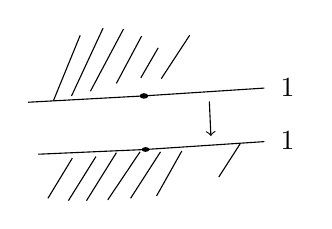
\begin{tikzpicture}[x=1cm,y=1cm]
\draw (0,1.0)--(1.46,1.08)--(3.0,1.18) (.13,.34)--(1.49,.40)--(3.00,.50);
\draw (.32,1.02)--(.66,1.85) (.55,1.08)--(.95,1.94) (.79,1.14)--(1.21,1.93) (1.12,1.24)--(1.44,1.84) (1.43,1.31)--(1.65,1.69) (1.69,1.30)--(2.05,1.85);
\draw (.56,.29)--(.25,-.22) (.86,.31)--(.51,-.25) (1.12,.36)--(.74,-.25) (1.42,.37)--(1.01,-.24) (1.68,.37)--(1.30,-.22) (1.95,.38)--(1.63,-.19) (2.69,.47)--(2.42,.05);
\draw[->] (2.30,1.01)--(2.32,.57);
\fill (1.47,1.08) ellipse (.055 and .035); \fill (1.49,.40) ellipse (.05 and .03);
\node[right] at (3.08,1.19) {$1$}; \node[right] at (3.08,.51) {$1$};
\end{tikzpicture}}

\figure{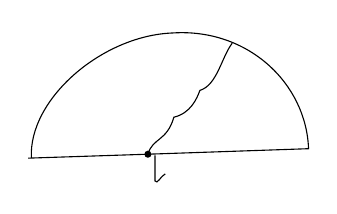
\begin{tikzpicture}[x=1cm,y=1cm]
\draw (0,0) .. controls (-.04,.75) and (.90,1.56) .. (1.80,1.59) .. controls (2.75,1.65) and (3.49,.95) .. (3.52,.12) -- (1.48,.05) -- (-.04,0);
\draw (1.48,.05) .. controls (1.54,.26) and (1.72,.21) .. (1.81,.52) .. controls (2.02,.57) and (2.10,.75) .. (2.14,.86) .. controls (2.36,.93) and (2.41,1.27) .. (2.55,1.46);
\fill (1.48,.05) circle (.045); \draw (1.57,.035)--(1.57,-.29) .. controls (1.60,-.34) and (1.64,-.23) .. (1.70,-.20);
\end{tikzpicture}}}

\uline{Lemme 3} Cas particuliers

a) Recollement de $H$ à $H$ \inserted{(\uline{deux exemplaires})} suivant un iso. rectifiable $[0,1]\overset{\sigma}{\longrightarrow}[0,1]$, regardé au voisinage de 0 [ou variante (\deleted{\unsure{mieux}} alors utiliser th. 3) : suivant un isom rectifiable $[-1,1]\overset{\sigma}{\longrightarrow}[-1,1]$, regardé au voisinage de 0].
% archive sheet number: 62
